\section{Lec 11}
\subsection{Covariant derivative - Connection}
In the last lecture we talked about the covariant derivative and we saw the version for the vector, for the dual vector, and how it transform between two coordinates systems. We constructed it so the output is a tensor, and we saw that even after changes of coordinates we still get a tensor.\par
The question now is, how to do
\[
\nabla _{\rho }T^{\mu _{1}\ldots \mu _{k}}_{\nu _{1}\ldots \nu _{l}} = ?
\]
The development is pretty boring but straight-forward:
\begin{equation}
= \partial_{\rho }T^{\mu_{1} \ldots \mu_{k}}_{\nu_{1} \ldots \nu_{l}} + \Gamma ^{\mu _{1}}_{\rho \alpha } T^{\alpha \mu_{2} \ldots \mu_{k}}_{\nu_{1} \ldots \nu_{l}} + \Gamma ^{\mu_{2}}_{\rho \alpha }T^{\mu_{1} \alpha \mu_{3} \ldots \mu_{k}}_{\nu_{1} \ldots \nu_{l}} + \ldots - \Gamma ^{\alpha }_{\mu \nu _{1}} T^{\mu _{1} \ldots \mu _{k}}_{\alpha \nu_{2} \ldots \nu_{l}} - \ldots 
\end{equation}
These $\Gamma $ connections are just tables of 64 entries of numbers, not tensors, and putting indices up and down to it it's abuse of notation. \par
Now we will make a couple of assumptions on the structure of $\Gamma $.
\subsubsection{Torsion}
\paragraph{Statement I} Given two different connections $\Gamma^{\mu }_{\alpha \beta }$ and $\tilde{\Gamma }^{\mu }_{\alpha \beta }$, we define
\[
S^{\mu }_{\alpha \beta } = \Gamma ^{\mu }_{\alpha \beta } - \tilde{\Gamma }^{\mu }_{\alpha \beta }	
\]
$\to  S^{\mu }_{\alpha \beta }$ is a (1,2) tensor. Why? Since I have
\[
\nabla _{\mu }V^{\nu } = \partial_{\mu }V^{\nu }+ \Gamma ^{\nu }_{\mu  \alpha }V^{\alpha }
\]
I can define a complement
\[
\tilde{\nabla }_{\mu }V^{\nu } = \partial_{\mu }V^{\nu } + \tilde{\Gamma }^{\nu }_{\mu \alpha }V^{\alpha }
\]
so i get
\[
\to  \nabla _{\mu }V^{\nu }- \tilde{\nabla }_{\mu }V^{\nu } = \left( \Gamma ^{\nu }_{\mu  \alpha } - \tilde{\Gamma }^{\nu }_{\mu  \alpha } \right)V^{\alpha } = S^{\nu }_{\mu  \alpha }V^{\alpha }
\]
and this is valid \emph{only} if $S^{\mu }_{\nu  \alpha }$ is a tensor.

\paragraph{Statement II} if $\Gamma ^{\mu }_{\alpha \beta }$ is a connection $\implies  \Gamma ^{\mu }_{\beta  \alpha }$ is a connection.\par
That's why we define the \emph{ Torsion tensor}
\[
	T^{\mu }_{\alpha \beta }\equiv \Gamma  ^{\mu }_{\alpha \beta } - \Gamma ^{\mu }_{\beta  \alpha } = 2 \Gamma ^{\mu }_{[\alpha \beta ]}
\]
The metric adopted in this course is a \emph{ Torsion-Free} metric, so the torsion tensor is vanishing.\par
How many entries do I have for a connection?
\[
\Gamma ^{\mu \to 4}_{\alpha \beta \to 10}
\]
so in total I have 40 entries, 4 for the upper index and 10 for the lowers because symmetry, \par

As we will see later, the name \emph{connection} comes from the fact that it is used to transport vectors from one tangent space to another.
\subsubsection{Metric Compatibility}
So, the torsion tensor is antisymmetric on its lower indices, and a connection that is symmetric on its lower indices is \emph{torsion-free}
We can define a unique connection on a manifold with metric $g_{\mu \nu }$ by introducing two additional properties, torsion-freeness and the metric compatibility.
The metric compatibility is a property of the covariant derivative and it's expressed as follows
\[
\nabla \rho g_{\mu \nu } = 0
\]
A connection is \emph{metric compatible} if the covariant derivative of the metric with respect to that connection is everywhere 0. \par
We want to see how this property works with the \emph{inverse metric tensor}, so let's start from
\begin{equation}
\nabla _{\rho } \left( g^{\alpha \beta } g_{\beta  \gamma } \right) =\nabla _{\rho } \left( \delta ^{\alpha }_{\gamma }  \right) = \Gamma ^{\alpha }_{\rho \lambda  }\delta^{\lambda }_{\gamma } - \Gamma ^{\sigma  }_{\rho \gamma }\delta^{\alpha }_{\sigma } + \partial_{\rho }\left( \delta ^{\alpha }_{\gamma } \right) = \left( \Gamma ^{\alpha }_{\rho  \gamma } - \Gamma ^{\alpha }_{\rho  \gamma } \right) = 0
\end{equation}
the term with the partial derivative cancels out because $\delta $ is constant, and we equal everything to zero because the covariant derivative of the Kronecker delta is 0. On the right side we can apply the Leibniz rule so
\begin{equation}
g^{\alpha \beta }\nabla _{\rho }\left( g_{\beta \gamma } \right) + \nabla _{\rho }\left( g^{\alpha \beta } \right)g_{\beta \gamma } = 0
\end{equation}
the first term is 0, because we said so, the connection is metric compatible. We are left with
\[
g_{\beta  \gamma }\nabla _{\rho }\left( g^{\alpha \beta } \right) = 0
\]
by multiplying on both sides $g^{\gamma \sigma }$
\[
g^{\gamma \sigma } g_{\beta \gamma } \nabla _{\rho } \left( g^{\alpha \beta } \right) =0
\]
I get
\[
\delta ^{\sigma }_{\beta }\nabla _{\rho }\left( g^{\alpha \beta } \right) = \nabla _{\rho }\left( \delta ^{\sigma }_{\beta } g^{\alpha \beta } \right) = \nabla _{\rho }\left( g^{\alpha \sigma } \right) = 0
\]
So, in conclusion the covariant derivative of the inverse of metric tensor is null. It was not trivial.

After this we can see that a metric-compatible covariant derivative commutes with raising and lowering of indices, so for a generic vector $V^{\nu }$
\[
\nabla _{\mu }V^{\nu } = g_{\alpha \nu }\nabla _{\mu }\left( v^{\mu } \right) = \nabla _{\mu }\left( g_{\alpha \nu }V^{\nu } \right) = \nabla _{\mu }V_{\nu }
\]

With non-metric compatible connections we would have to be very careful about index placement wen taking a covariant derivative. \par
There is exactly one torsion-free connection on a manifold that is compatible with some generic metric on that manifold. \par

We can demonstrate \emph{existence} and \emph{uniqueness} by deriving a manifestly unique expression for the connection coefficients in terms of the metric, so we will expand the equation of metric compatibility for three different permutations of the indices.
\begin{gather*}
\nabla _{\rho }g_{\mu \nu } = \partial_{\rho }g_{\mu \nu } - \Gamma ^{\lambda }_{\rho \mu }g_{ \lambda \nu  } - \Gamma ^{\lambda }_{\rho \nu } g_{\mu \lambda }=0  \text{ (a) }\\
\nabla _{\mu }g_{\nu \rho } = \partial_{\mu }g_{\nu \rho } - \Gamma ^{\lambda }_{\mu \nu }g_{\lambda \rho } - \Gamma ^{\lambda }_{\mu \rho }g_{\nu \lambda } =0 \text{ (b) }\\
\nabla _{\nu }g_{\rho \mu } = \partial_{\nu }g_{\rho \mu } - \Gamma ^{\lambda }_{\nu \rho } g_{\lambda \mu } - \Gamma ^{\lambda }_{\nu \mu } g_{\rho  \lambda } = 0 \text{ (c) }
\end{gather*}
we see that \emph{(a)-(b)-(c) = 0}, and it is obvious because individually they're equal to 0. \par
But let's see in detail what's happening
\begin{gather*}
\partial_{\rho }g_{\mu \nu } - \partial_{\mu }g_{\nu \rho } - \partial_{\nu }g_{\rho \mu } - \colorbox{yellow}{$ \Gamma^{\alpha }_{\rho \mu }g_{\alpha \nu }  $} - \colorbox{green}{$ \Gamma ^{\alpha }_{\rho \nu }g_{\mu \alpha }  $} + \\
 + \Gamma ^{\alpha }_{\mu \nu }g_{\alpha \rho } + \colorbox{yellow}{$ \Gamma^{\alpha }_{\mu \rho }g_{\nu \alpha }  $} + \colorbox{green}{$ \Gamma ^{\alpha }_{\nu \rho }g_{\alpha \mu }  $} + \Gamma ^{\alpha }_{\nu \mu }g_{\rho \alpha } = 0 \\
\end{gather*}
 We subtract the highlighted ones and use the symmetry of the connection to get
 \[
 2g_{\rho \alpha }\Gamma ^{\alpha }_{\mu \nu } - \partial_{\mu }g_{\nu \rho } + \partial_{\nu }g_{\mu \rho } - \partial_{\rho }g_{\mu \nu }
 \]
 We multiply both sides by $g^{\rho \sigma }$	
\begin{equation}
	\Gamma^{\sigma }_{\mu \nu } = \frac{1}{2} g^{\rho \sigma } [\partial_{\mu } g_{\nu \rho } + \partial_{\nu } g_{\mu \rho } - \partial_{\rho }g_{\mu \nu } ]
\end{equation}
 This is one of the most important expressions of the course. \par
 We have seen that a flat spacetime has a Minkowski metric everywhere. \par
 But how to define curvature? \par
 The fact that $g_{\mu \nu }$ depends on the coordinates is not enough (e.g. spherical coordinates). But now we have a new object\par
 Let's think a little bit: in flat spacetime if $\partial \leftrightarrow \nabla $ and this $\implies \Gamma  = 0$. Is that true? \par
 
 In 3D coordinates, using other coordinates, do connections have to be 0? Be
 \[
 \overline{\nabla } = \left( \frac{\partial }{\partial x} , \frac{\partial }{\partial y}  \right)
 \]
 that's the gradient in cartesian coordinates, but in polar coordinates
 \[
 = \left( \frac{\partial }{\partial r} , \frac{1}{r} \frac{\partial }{\partial \theta }  \right)
 \]
 I can compute the additional factor with christoffel symbols.
 Take $ds^{2} = dr^{2} + r^{2}d\theta ^{2}$, polar coordinates on plane, and compute the christoffel symbol. How many entries?
 \[
 \Gamma ^{\alpha \to 2}_{\beta \gamma \to 3} 
 \]
 I don't remember what the professor was trying to say but in doubt see Carroll.

 \subsection{Parallel Transport}
 


\tikzset{every picture/.style={line width=0.75pt}} %set default line width to 0.75pt        

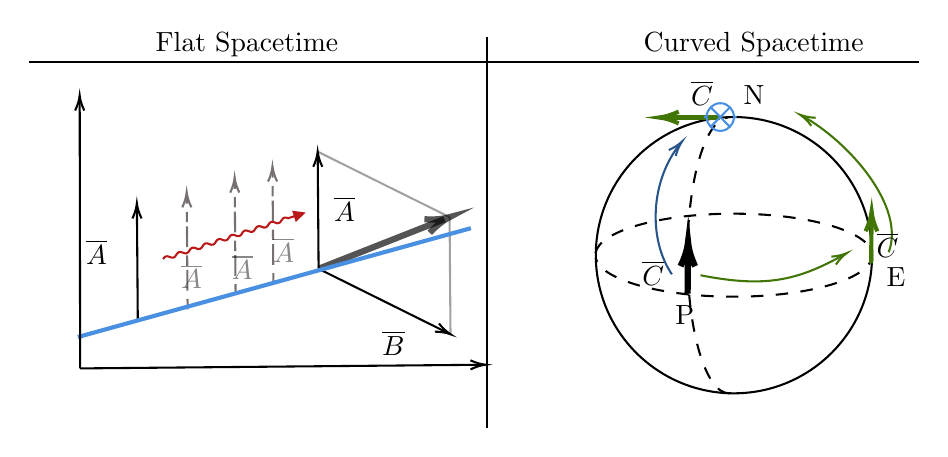
\begin{tikzpicture}[x=0.50pt,y=0.50pt,yscale=-1,xscale=1]
%uncomment if require: \path (0,300); %set diagram left start at 0, and has height of 300

%Straight Lines [id:da7804419238627388] 
\draw    (350.5,11.25) -- (350.5,294) ;
%Straight Lines [id:da6280355665081884] 
\draw    (19.5,29.25) -- (663,29.25) ;
%Straight Lines [id:da4130726982439956] 
\draw    (98.33,216.33) -- (97.68,133.67) ;
\draw [shift={(97.67,131.67)}, rotate = 89.55] [color={rgb, 255:red, 0; green, 0; blue, 0 }  ][line width=0.75]    (10.93,-3.29) .. controls (6.95,-1.4) and (3.31,-0.3) .. (0,0) .. controls (3.31,0.3) and (6.95,1.4) .. (10.93,3.29)   ;
%Straight Lines [id:da4487944386747611] 
\draw    (229,179) -- (228.35,96.33) ;
\draw [shift={(228.33,94.33)}, rotate = 89.55] [color={rgb, 255:red, 0; green, 0; blue, 0 }  ][line width=0.75]    (10.93,-3.29) .. controls (6.95,-1.4) and (3.31,-0.3) .. (0,0) .. controls (3.31,0.3) and (6.95,1.4) .. (10.93,3.29)   ;
%Straight Lines [id:da34584707728272546] 
\draw [color={rgb, 255:red, 118; green, 112; blue, 112 }  ,draw opacity=1 ] [dash pattern={on 3.75pt off 3pt on 7.5pt off 1.5pt}]  (134.33,208.33) -- (133.68,125.67) ;
\draw [shift={(133.67,123.67)}, rotate = 89.55] [color={rgb, 255:red, 118; green, 112; blue, 112 }  ,draw opacity=1 ][line width=0.75]    (10.93,-3.29) .. controls (6.95,-1.4) and (3.31,-0.3) .. (0,0) .. controls (3.31,0.3) and (6.95,1.4) .. (10.93,3.29)   ;
%Straight Lines [id:da8607896715027422] 
\draw [color={rgb, 255:red, 118; green, 112; blue, 112 }  ,draw opacity=1 ] [dash pattern={on 3.75pt off 3pt on 7.5pt off 1.5pt}]  (169,197.67) -- (168.35,115) ;
\draw [shift={(168.33,113)}, rotate = 89.55] [color={rgb, 255:red, 118; green, 112; blue, 112 }  ,draw opacity=1 ][line width=0.75]    (10.93,-3.29) .. controls (6.95,-1.4) and (3.31,-0.3) .. (0,0) .. controls (3.31,0.3) and (6.95,1.4) .. (10.93,3.29)   ;
%Straight Lines [id:da18547678451320238] 
\draw [color={rgb, 255:red, 118; green, 112; blue, 112 }  ,draw opacity=1 ] [dash pattern={on 3.75pt off 3pt on 7.5pt off 1.5pt}]  (196.33,189.67) -- (195.68,107) ;
\draw [shift={(195.67,105)}, rotate = 89.55] [color={rgb, 255:red, 118; green, 112; blue, 112 }  ,draw opacity=1 ][line width=0.75]    (10.93,-3.29) .. controls (6.95,-1.4) and (3.31,-0.3) .. (0,0) .. controls (3.31,0.3) and (6.95,1.4) .. (10.93,3.29)   ;
%Straight Lines [id:da6531580304035787] 
\draw [color={rgb, 255:red, 186; green, 25; blue, 25 }  ,draw opacity=1 ]   (116.67,172) .. controls (117.74,169.9) and (119.32,169.38) .. (121.42,170.45) .. controls (123.53,171.52) and (125.11,171) .. (126.17,168.89) .. controls (127.24,166.79) and (128.82,166.27) .. (130.92,167.34) .. controls (133.02,168.41) and (134.61,167.89) .. (135.68,165.79) .. controls (136.74,163.68) and (138.32,163.16) .. (140.43,164.23) .. controls (142.53,165.3) and (144.11,164.78) .. (145.18,162.68) .. controls (146.25,160.58) and (147.83,160.06) .. (149.93,161.13) .. controls (152.04,162.2) and (153.62,161.68) .. (154.69,159.57) .. controls (155.76,157.47) and (157.34,156.95) .. (159.44,158.02) .. controls (161.54,159.09) and (163.12,158.57) .. (164.19,156.47) .. controls (165.25,154.36) and (166.83,153.84) .. (168.94,154.91) .. controls (171.04,155.98) and (172.63,155.46) .. (173.7,153.36) .. controls (174.77,151.26) and (176.35,150.74) .. (178.45,151.81) .. controls (180.56,152.88) and (182.14,152.36) .. (183.2,150.25) .. controls (184.27,148.15) and (185.86,147.63) .. (187.96,148.7) .. controls (190.06,149.77) and (191.64,149.25) .. (192.71,147.15) .. controls (193.77,145.04) and (195.35,144.52) .. (197.46,145.59) .. controls (199.56,146.66) and (201.14,146.14) .. (202.21,144.04) .. controls (203.28,141.93) and (204.86,141.41) .. (206.97,142.48) -- (209.21,141.75) -- (216.82,139.27) ;
\draw [shift={(219.67,138.33)}, rotate = 161.9] [fill={rgb, 255:red, 186; green, 25; blue, 25 }  ,fill opacity=1 ][line width=0.08]  [draw opacity=0] (8.93,-4.29) -- (0,0) -- (8.93,4.29) -- cycle    ;
%Straight Lines [id:da096404784455415] 
\draw    (229,179) -- (322.54,225.44) ;
\draw [shift={(324.33,226.33)}, rotate = 206.4] [color={rgb, 255:red, 0; green, 0; blue, 0 }  ][line width=0.75]    (10.93,-3.29) .. controls (6.95,-1.4) and (3.31,-0.3) .. (0,0) .. controls (3.31,0.3) and (6.95,1.4) .. (10.93,3.29)   ;
%Straight Lines [id:da31708594059819595] 
\draw [color={rgb, 255:red, 0; green, 0; blue, 0 }  ,draw opacity=0.37 ]   (228.33,94.33) -- (323.67,141.67) ;
%Straight Lines [id:da44013896128415253] 
\draw [color={rgb, 255:red, 0; green, 0; blue, 0 }  ,draw opacity=0.37 ]   (324.33,226.33) -- (323.67,141.67) ;
%Straight Lines [id:da693791852252502] 
\draw [color={rgb, 255:red, 0; green, 0; blue, 0 }  ,draw opacity=0.67 ][line width=2.25]    (229,179) -- (319.95,143.13) ;
\draw [shift={(323.67,141.67)}, rotate = 158.48] [color={rgb, 255:red, 0; green, 0; blue, 0 }  ,draw opacity=0.67 ][line width=2.25]    (17.49,-5.26) .. controls (11.12,-2.23) and (5.29,-0.48) .. (0,0) .. controls (5.29,0.48) and (11.12,2.23) .. (17.49,5.26)   ;
%Shape: Circle [id:dp9665324253206228] 
\draw   (429.33,169.17) .. controls (429.33,114.03) and (474.03,69.33) .. (529.17,69.33) .. controls (584.3,69.33) and (629,114.03) .. (629,169.17) .. controls (629,224.3) and (584.3,269) .. (529.17,269) .. controls (474.03,269) and (429.33,224.3) .. (429.33,169.17) -- cycle ;
%Shape: Arc [id:dp9307781681306638] 
\draw  [draw opacity=0][dash pattern={on 4.5pt off 4.5pt}] (429.12,167.7) .. controls (431.66,151.81) and (475.41,139.17) .. (529,139.17) .. controls (584.23,139.17) and (629,152.6) .. (629,169.17) .. controls (629,185.74) and (584.23,199.17) .. (529,199.17) .. controls (475.9,199.17) and (432.46,186.75) .. (429.2,171.07) -- (529,169.17) -- cycle ; \draw  [dash pattern={on 4.5pt off 4.5pt}] (429.12,167.7) .. controls (431.66,151.81) and (475.41,139.17) .. (529,139.17) .. controls (584.23,139.17) and (629,152.6) .. (629,169.17) .. controls (629,185.74) and (584.23,199.17) .. (529,199.17) .. controls (475.9,199.17) and (432.46,186.75) .. (429.2,171.07) ;  
%Shape: Arc [id:dp9109349274225841] 
\draw  [draw opacity=0][dash pattern={on 4.5pt off 4.5pt}] (525.66,269) .. controls (525.63,269) and (525.6,269) .. (525.57,269) .. controls (509,269) and (495.57,224.35) .. (495.57,169.27) .. controls (495.57,114.74) and (508.73,70.44) .. (525.07,69.55) -- (525.57,169.27) -- cycle ; \draw  [dash pattern={on 4.5pt off 4.5pt}] (525.66,269) .. controls (525.63,269) and (525.6,269) .. (525.57,269) .. controls (509,269) and (495.57,224.35) .. (495.57,169.27) .. controls (495.57,114.74) and (508.73,70.44) .. (525.07,69.55) ;  
%Straight Lines [id:da9377226925217493] 
\draw [line width=2.25]    (495.67,197) -- (495.96,163.67) ;
\draw [shift={(496,159.67)}, rotate = 90.51] [color={rgb, 255:red, 0; green, 0; blue, 0 }  ][line width=2.25]    (17.49,-5.26) .. controls (11.12,-2.23) and (5.29,-0.48) .. (0,0) .. controls (5.29,0.48) and (11.12,2.23) .. (17.49,5.26)   ;
%Curve Lines [id:da248689634217361] 
\draw [color={rgb, 255:red, 65; green, 117; blue, 5 }  ,draw opacity=1 ]   (505,183.67) .. controls (551.62,192.86) and (574.96,187.82) .. (609.1,168.56) ;
\draw [shift={(610.67,167.67)}, rotate = 150.26] [color={rgb, 255:red, 65; green, 117; blue, 5 }  ,draw opacity=1 ][line width=0.75]    (10.93,-3.29) .. controls (6.95,-1.4) and (3.31,-0.3) .. (0,0) .. controls (3.31,0.3) and (6.95,1.4) .. (10.93,3.29)   ;
%Curve Lines [id:da3715785341810326] 
\draw [color={rgb, 255:red, 40; green, 85; blue, 139 }  ,draw opacity=1 ]   (484.33,183) .. controls (467.26,158.05) and (468.3,115.63) .. (490.63,88.24) ;
\draw [shift={(491.67,87)}, rotate = 130.49] [color={rgb, 255:red, 40; green, 85; blue, 139 }  ,draw opacity=1 ][line width=0.75]    (10.93,-3.29) .. controls (6.95,-1.4) and (3.31,-0.3) .. (0,0) .. controls (3.31,0.3) and (6.95,1.4) .. (10.93,3.29)   ;
%Curve Lines [id:da33000822429954535] 
\draw [color={rgb, 255:red, 65; green, 117; blue, 5 }  ,draw opacity=1 ]   (641,167) .. controls (653.48,134.17) and (612.27,87.1) .. (578.54,68.5) ;
\draw [shift={(577,67.67)}, rotate = 27.9] [color={rgb, 255:red, 65; green, 117; blue, 5 }  ,draw opacity=1 ][line width=0.75]    (10.93,-3.29) .. controls (6.95,-1.4) and (3.31,-0.3) .. (0,0) .. controls (3.31,0.3) and (6.95,1.4) .. (10.93,3.29)   ;
%Straight Lines [id:da11933692361161596] 
\draw [color={rgb, 255:red, 65; green, 117; blue, 5 }  ,draw opacity=1 ][line width=1.5]    (628.33,175) -- (628.64,140.67) ;
\draw [shift={(628.67,137.67)}, rotate = 90.51] [color={rgb, 255:red, 65; green, 117; blue, 5 }  ,draw opacity=1 ][line width=1.5]    (14.21,-4.28) .. controls (9.04,-1.82) and (4.3,-0.39) .. (0,0) .. controls (4.3,0.39) and (9.04,1.82) .. (14.21,4.28)   ;
%Straight Lines [id:da9460218080051334] 
\draw [color={rgb, 255:red, 65; green, 117; blue, 5 }  ,draw opacity=1 ][line width=1.5]    (519,69.67) -- (478,69.67) ;
\draw [shift={(475,69.67)}, rotate = 360] [color={rgb, 255:red, 65; green, 117; blue, 5 }  ,draw opacity=1 ][line width=1.5]    (14.21,-4.28) .. controls (9.04,-1.82) and (4.3,-0.39) .. (0,0) .. controls (4.3,0.39) and (9.04,1.82) .. (14.21,4.28)   ;
%Shape: Light Bulb [id:dp7648536590068119] 
\draw  [color={rgb, 255:red, 74; green, 144; blue, 226 }  ,draw opacity=1 ] (509.44,69.33) .. controls (509.44,63.81) and (513.86,59.33) .. (519.31,59.33) .. controls (524.75,59.33) and (529.17,63.81) .. (529.17,69.33) .. controls (529.17,74.86) and (524.75,79.33) .. (519.31,79.33) .. controls (513.86,79.33) and (509.44,74.86) .. (509.44,69.33) -- cycle (512.28,62.21) -- (526.33,76.45) (526.33,62.21) -- (512.28,76.45) (507.47,69.33) -- (509.44,69.33) (529.17,69.33) -- (531.14,69.33) ;
%Straight Lines [id:da26085572297009496] 
\draw [color={rgb, 255:red, 74; green, 144; blue, 226 }  ,draw opacity=1 ][line width=1.5]    (55,228.33) -- (339,149.67) ;
%Straight Lines [id:da17265066162065923] 
\draw    (56.67,251) -- (56.34,55.67) ;
\draw [shift={(56.33,53.67)}, rotate = 89.9] [color={rgb, 255:red, 0; green, 0; blue, 0 }  ][line width=0.75]    (10.93,-3.29) .. controls (6.95,-1.4) and (3.31,-0.3) .. (0,0) .. controls (3.31,0.3) and (6.95,1.4) .. (10.93,3.29)   ;
%Straight Lines [id:da8026826708800486] 
\draw    (56.67,251) -- (347.67,248.35) ;
\draw [shift={(349.67,248.33)}, rotate = 179.48] [color={rgb, 255:red, 0; green, 0; blue, 0 }  ][line width=0.75]    (10.93,-3.29) .. controls (6.95,-1.4) and (3.31,-0.3) .. (0,0) .. controls (3.31,0.3) and (6.95,1.4) .. (10.93,3.29)   ;

% Text Node
\draw (109,5.5) node [anchor=north west][inner sep=0.75pt]   [align=left] {Flat Spacetime};
% Text Node
\draw (461.67,5.67) node [anchor=north west][inner sep=0.75pt]   [align=left] {Curved Spacetime};
% Text Node
\draw (58.67,155.67) node [anchor=north west][inner sep=0.75pt]   [align=left] {$\displaystyle \overline{A}$};
% Text Node
\draw (238,125) node [anchor=north west][inner sep=0.75pt]   [align=left] {$\displaystyle \overline{A}$};
% Text Node
\draw (127.33,173.67) node [anchor=north west][inner sep=0.75pt]  [color={rgb, 255:red, 0; green, 0; blue, 0 }  ,opacity=0.47 ] [align=left] {$\displaystyle \overline{A}$};
% Text Node
\draw (164,167) node [anchor=north west][inner sep=0.75pt]  [color={rgb, 255:red, 0; green, 0; blue, 0 }  ,opacity=0.47 ] [align=left] {$\displaystyle \overline{A}$};
% Text Node
\draw (194,154.33) node [anchor=north west][inner sep=0.75pt]  [color={rgb, 255:red, 0; green, 0; blue, 0 }  ,opacity=0.47 ] [align=left] {$\displaystyle \overline{A}$};
% Text Node
\draw (272.67,221.67) node [anchor=north west][inner sep=0.75pt]   [align=left] {$\displaystyle \overline{B}$};
% Text Node
\draw (484.67,203) node [anchor=north west][inner sep=0.75pt]   [align=left] {P};
% Text Node
\draw (534,44.67) node [anchor=north west][inner sep=0.75pt]   [align=left] {N};
% Text Node
\draw (637.33,176) node [anchor=north west][inner sep=0.75pt]   [align=left] {E};
% Text Node
\draw (460.67,171) node [anchor=north west][inner sep=0.75pt]   [align=left] {$\displaystyle \overline{C}$};
% Text Node
\draw (630,151) node [anchor=north west][inner sep=0.75pt]   [align=left] {$\displaystyle \overline{C}$};
% Text Node
\draw (496,41) node [anchor=north west][inner sep=0.75pt]   [align=left] {$\displaystyle \overline{C}$};
\end{tikzpicture}

In flat spacetime, if we want to add $\overline{A}+ \overline{B}$, we move the $\overline{A}$ vector along the blue line. We \emph{can} move $\overline{A}$ also along a non-straight line but $\overline{A}$ remains $\overline{A}$, and for the sum I get the same result.\par
In flat spacetime parallel transport does not depend on the path.\par

In curved spacetime, if I move $\overline{C}$ from \emph{P} to \emph{N} along the geodesic, we get that $\overline{C}$ points inside the sheet. But if I choose another path like \emph{P-E-N}, then the outcome is a vector $\overline{C}$ that points toward left. It's not the same vector. \par
In curved spacetime parallel transport depends on the trajectory, we have to specify the path.\par
Be the path $x^{\mu }\left( \lambda  \right) : \mathbb{R} \to \text{ spacetime coordinates }$. In FST parallel transportation of a generic tensor is
\[
\frac{d}{d\lambda } \left( T^{\mu _{1} \ldots \mu _{l}}_{\nu _{1}\ldots \nu _{l}} \right) = 0
\]
and the first factor is the directional derivative. Or
\[
\frac{d x^{\sigma }}{d \lambda } \partial_{\sigma } \left( T^{\mu _{1}\ldots \mu _{k}}_{\nu _{1}\ldots \nu _{l}} \right) = 0
\]
While in CST:
\[
\frac{dx^{\sigma }}{d\lambda } \nabla _{\sigma } \left(T^{\mu _{1}\ldots \mu _{k}}_{\nu _{1}\ldots \nu _{l}} \right) = 0
\]
Let's see a simple example: imagine we have $x^{\mu }\left( \lambda  \right) = \left( \lambda , 0, 0 , 0 \right)$ so $x^{\mu }\left( 0 \right) = \left( 0,0,0,0 \right)$ and the four velocity is $V^{\mu }\left( 0 \right) = \left( 1,0,0,0 \right)$.
In FST 
\[
\frac{dx^{\sigma }}{d\lambda } \left( \partial_{\sigma }V^{\mu } \right) = \frac{dx^{0}}{d\lambda } \partial_{0}V^{\mu } = \partial_{0}V^{\mu } = 0
\]
The vector does not change. \par

Why is it useful? Let's introduce
\subsubsection{Geodesics}
They are a straight line in curved space, the trajectory of a particle only subject to gravity. With \emph{straight line} we mean the path that is parallel transported along it's tangent vector.

\textbf{Example} In FST we have a vector that have the same direction of a straight line, and we want to move it along that line. 
So if I transport the vector tangent to the line, I get the same line.

\tikzset{every picture/.style={line width=0.75pt}}\label{imm:straigthline}

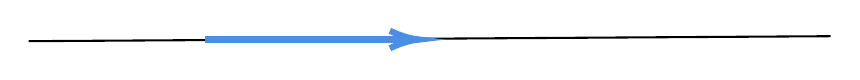
\begin{tikzpicture}[x=0.60pt,y=0.60pt,yscale=-1,xscale=1]
%uncomment if require: \path (0,300); %set diagram left start at 0, and has height of 300

%Straight Lines [id:da7933369365137976]
\draw    (100,106) -- (583,103) ;
%Straight Lines [id:da5367435588258249]
\draw [color={rgb, 255:red, 74; green, 144; blue, 226 }  ,draw opacity=1 ][line width=2.25]    (206,105) -- (331,105) ;
\draw [shift={(335,105)}, rotate = 180] [color={rgb, 255:red, 74; green, 144; blue, 226 }  ,draw opacity=1 ][line width=2.25]    (17.49,-5.26) .. controls (11.12,-2.23) and (5.29,-0.48) .. (0,0) .. controls (5.29,0.48) and (11.12,2.23) .. (17.49,5.26)   ;
\end{tikzpicture} \par
In CST, with path $x^{\mu }\left( \lambda  \right)$, we have tangent
\[
\frac{dx^{\mu }}{d\lambda  }
\]
and that gives
\[
\frac{dx^{\sigma }}{d\lambda } \nabla _{\sigma } \left( \frac{dx^{\mu }}{d\lambda } \right) = 0
\]
It's a geodesics if this last condition is satisfied.
Let's focus on this
\begin{gather*}
	\frac{dx^{\sigma }}{d\lambda } \left[ \frac{\partial }{\partial x^{\sigma }}  \frac{dx^{\mu }}{d\lambda } + \Gamma ^{\mu }_{\sigma \alpha } \frac{dx^{\alpha }}{d\lambda }\right] = 0 \\
\to  \frac{d^{2}x^{\mu }}{d\lambda } + \Gamma^{\mu }_{\alpha \beta } \frac{dx^{\alpha }}{d\lambda } \frac{d x^{\beta }}{d\lambda } = 0
\end{gather*}
the last one is the \emph{geodesics equation}, and it's very important. \par

Suggested exercise: do that in polar coordinates in FST.















